Hotspotizer has been developed through a process that utilizes user-centered design tools, in order to fulfill the needs of end-users. The choice of methods employed for the design work was influenced by methods used in previously published research on similar software \parencite{Ashbrook:2010, Lu:2012, Lu:2013, Kin:2012, Long:1999, Reis:2012}. This section describes the evolution of Hotspotizer; the evaluation of the final prototype; and insights gained throughout design, development, and deployment. Figure~\ref{fig:timeline} depicts a summary of the design and development processes on a timeline.

\begin{figure}[b]
\centering
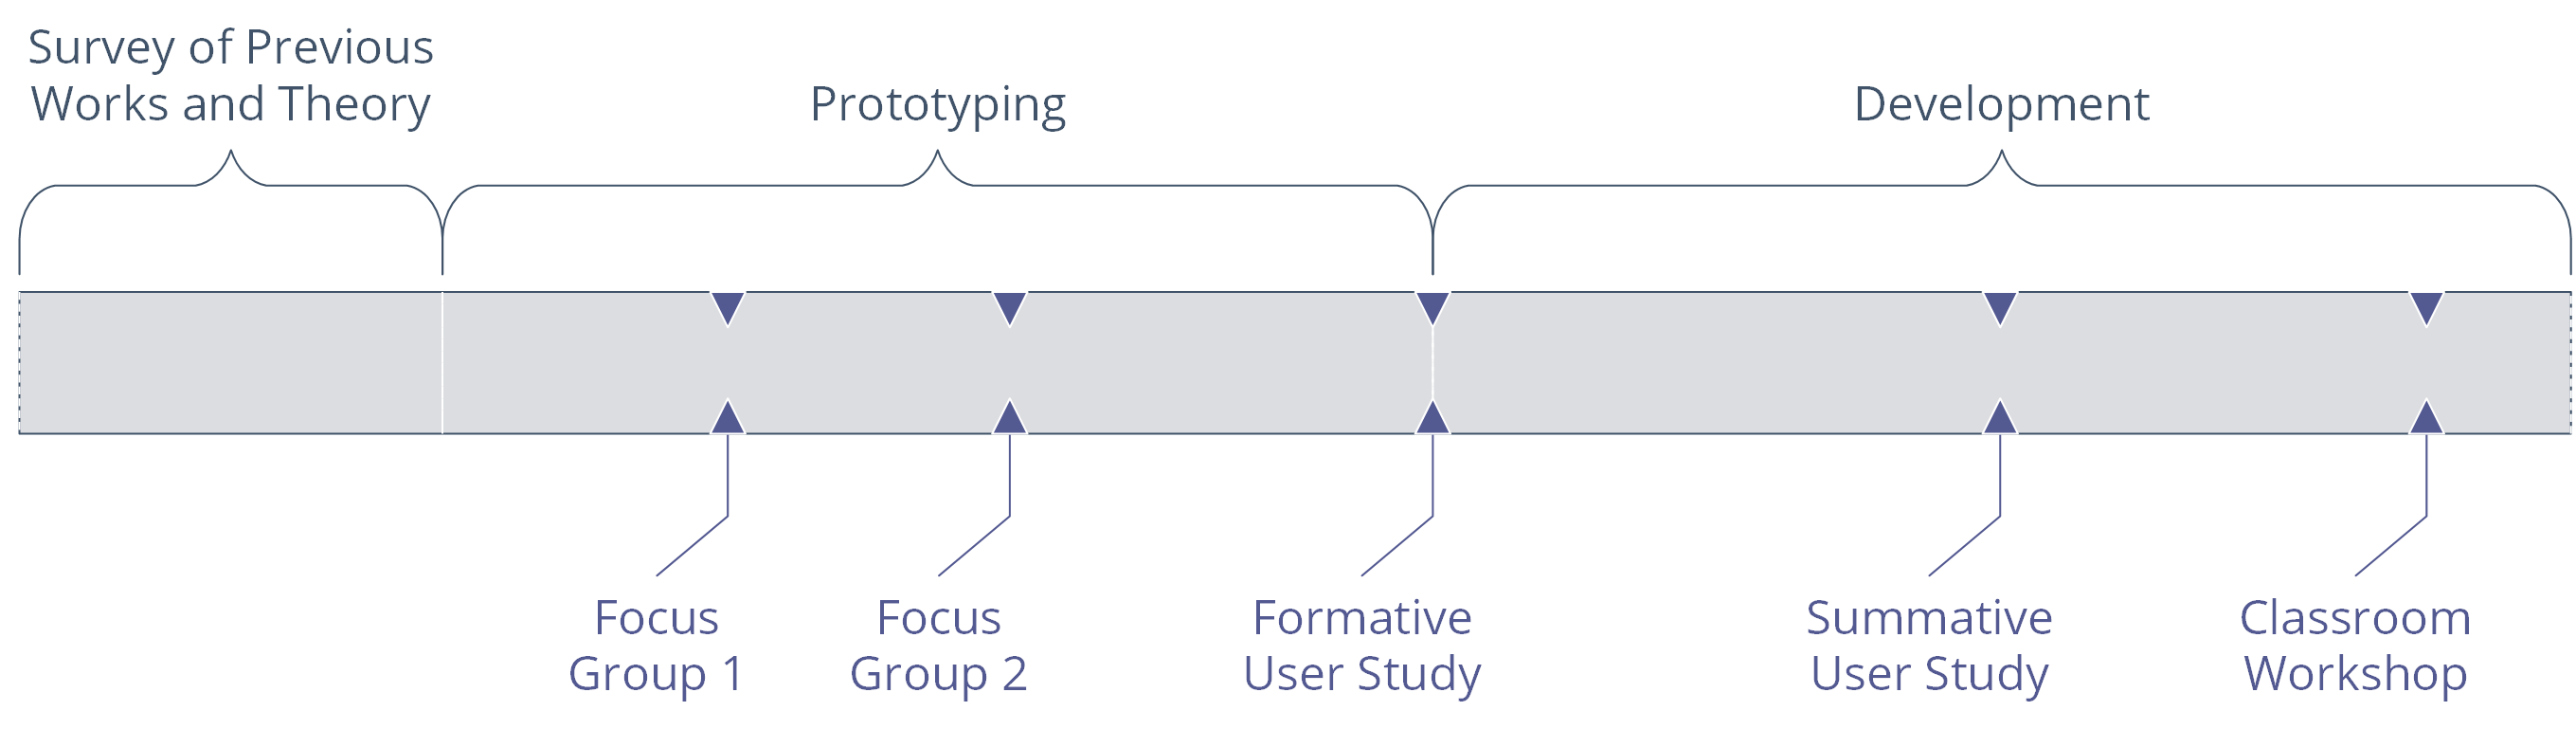
\includegraphics[width=\textwidth]{timeline}
\caption{A summary of the design and development processes.}
\label{fig:timeline}
\end{figure}

\section{Formative Studies}
\label{sec:formative-studies}

In the early stages of the design work for a tool to support authoring mid-air gestural interactions, the motivating question was \hl{\emph{what} to build.} The expected outcome from this stage --- which \textcite{Klemmer:2014} calls "needfinding" --- is the identification of the desiderata and the core features for the gesture authoring interface. To this end, two focus group meetings were conducted with a representative sample of end-users. The knowledge derived from the focus groups, along with insights from related work and analysis of related artifacts (described in Section~\ref{sec:authoring-mid-air-gestures}) informed subsequent design work. The later stages of development are described in Section~\ref{sec:summative-studies}.

\subsection{Focus Groups}

For user interface design, focus groups are a technique that can be used before higher fidelity design and development work to elicit user wants and needs \parencite{Nielsen:1997}. The nature of focus groups is informal and the results are generally qualitative. Focus groups have limited power, precision and accuracy due to methodological issues \parencite{Smithson:2000, Franz:2011}; but they are recommended as an initial needfinding strategy in the pursuit of open-ended questions \parencite{Nielsen:1997, Kitzinger:1995, Morgan:1996}.

\textcite{Nielsen:1997} recommends "exposing users to the most concrete examples of the technology being discussed" to improve the accuracy of the data gathered during focus groups. Per his advice, discussions during the focus group meetings were facilitated using various prototypes of different levels of fidelity. Initially, concepts were produced in the form of rough sketches and paper prototypes. During a second focus group meeting, a second round of prototypes of varying fidelity were used, which included video sketches and interactive user interface prototypes built using the \emph{Processing}\footnote{\href{http://www.processing.org}{processing.org}} programming language. Figure~\ref{fig:sketches-prototypes} shows samples from these preliminary renderings.

\begin{figure}[t]
\centering
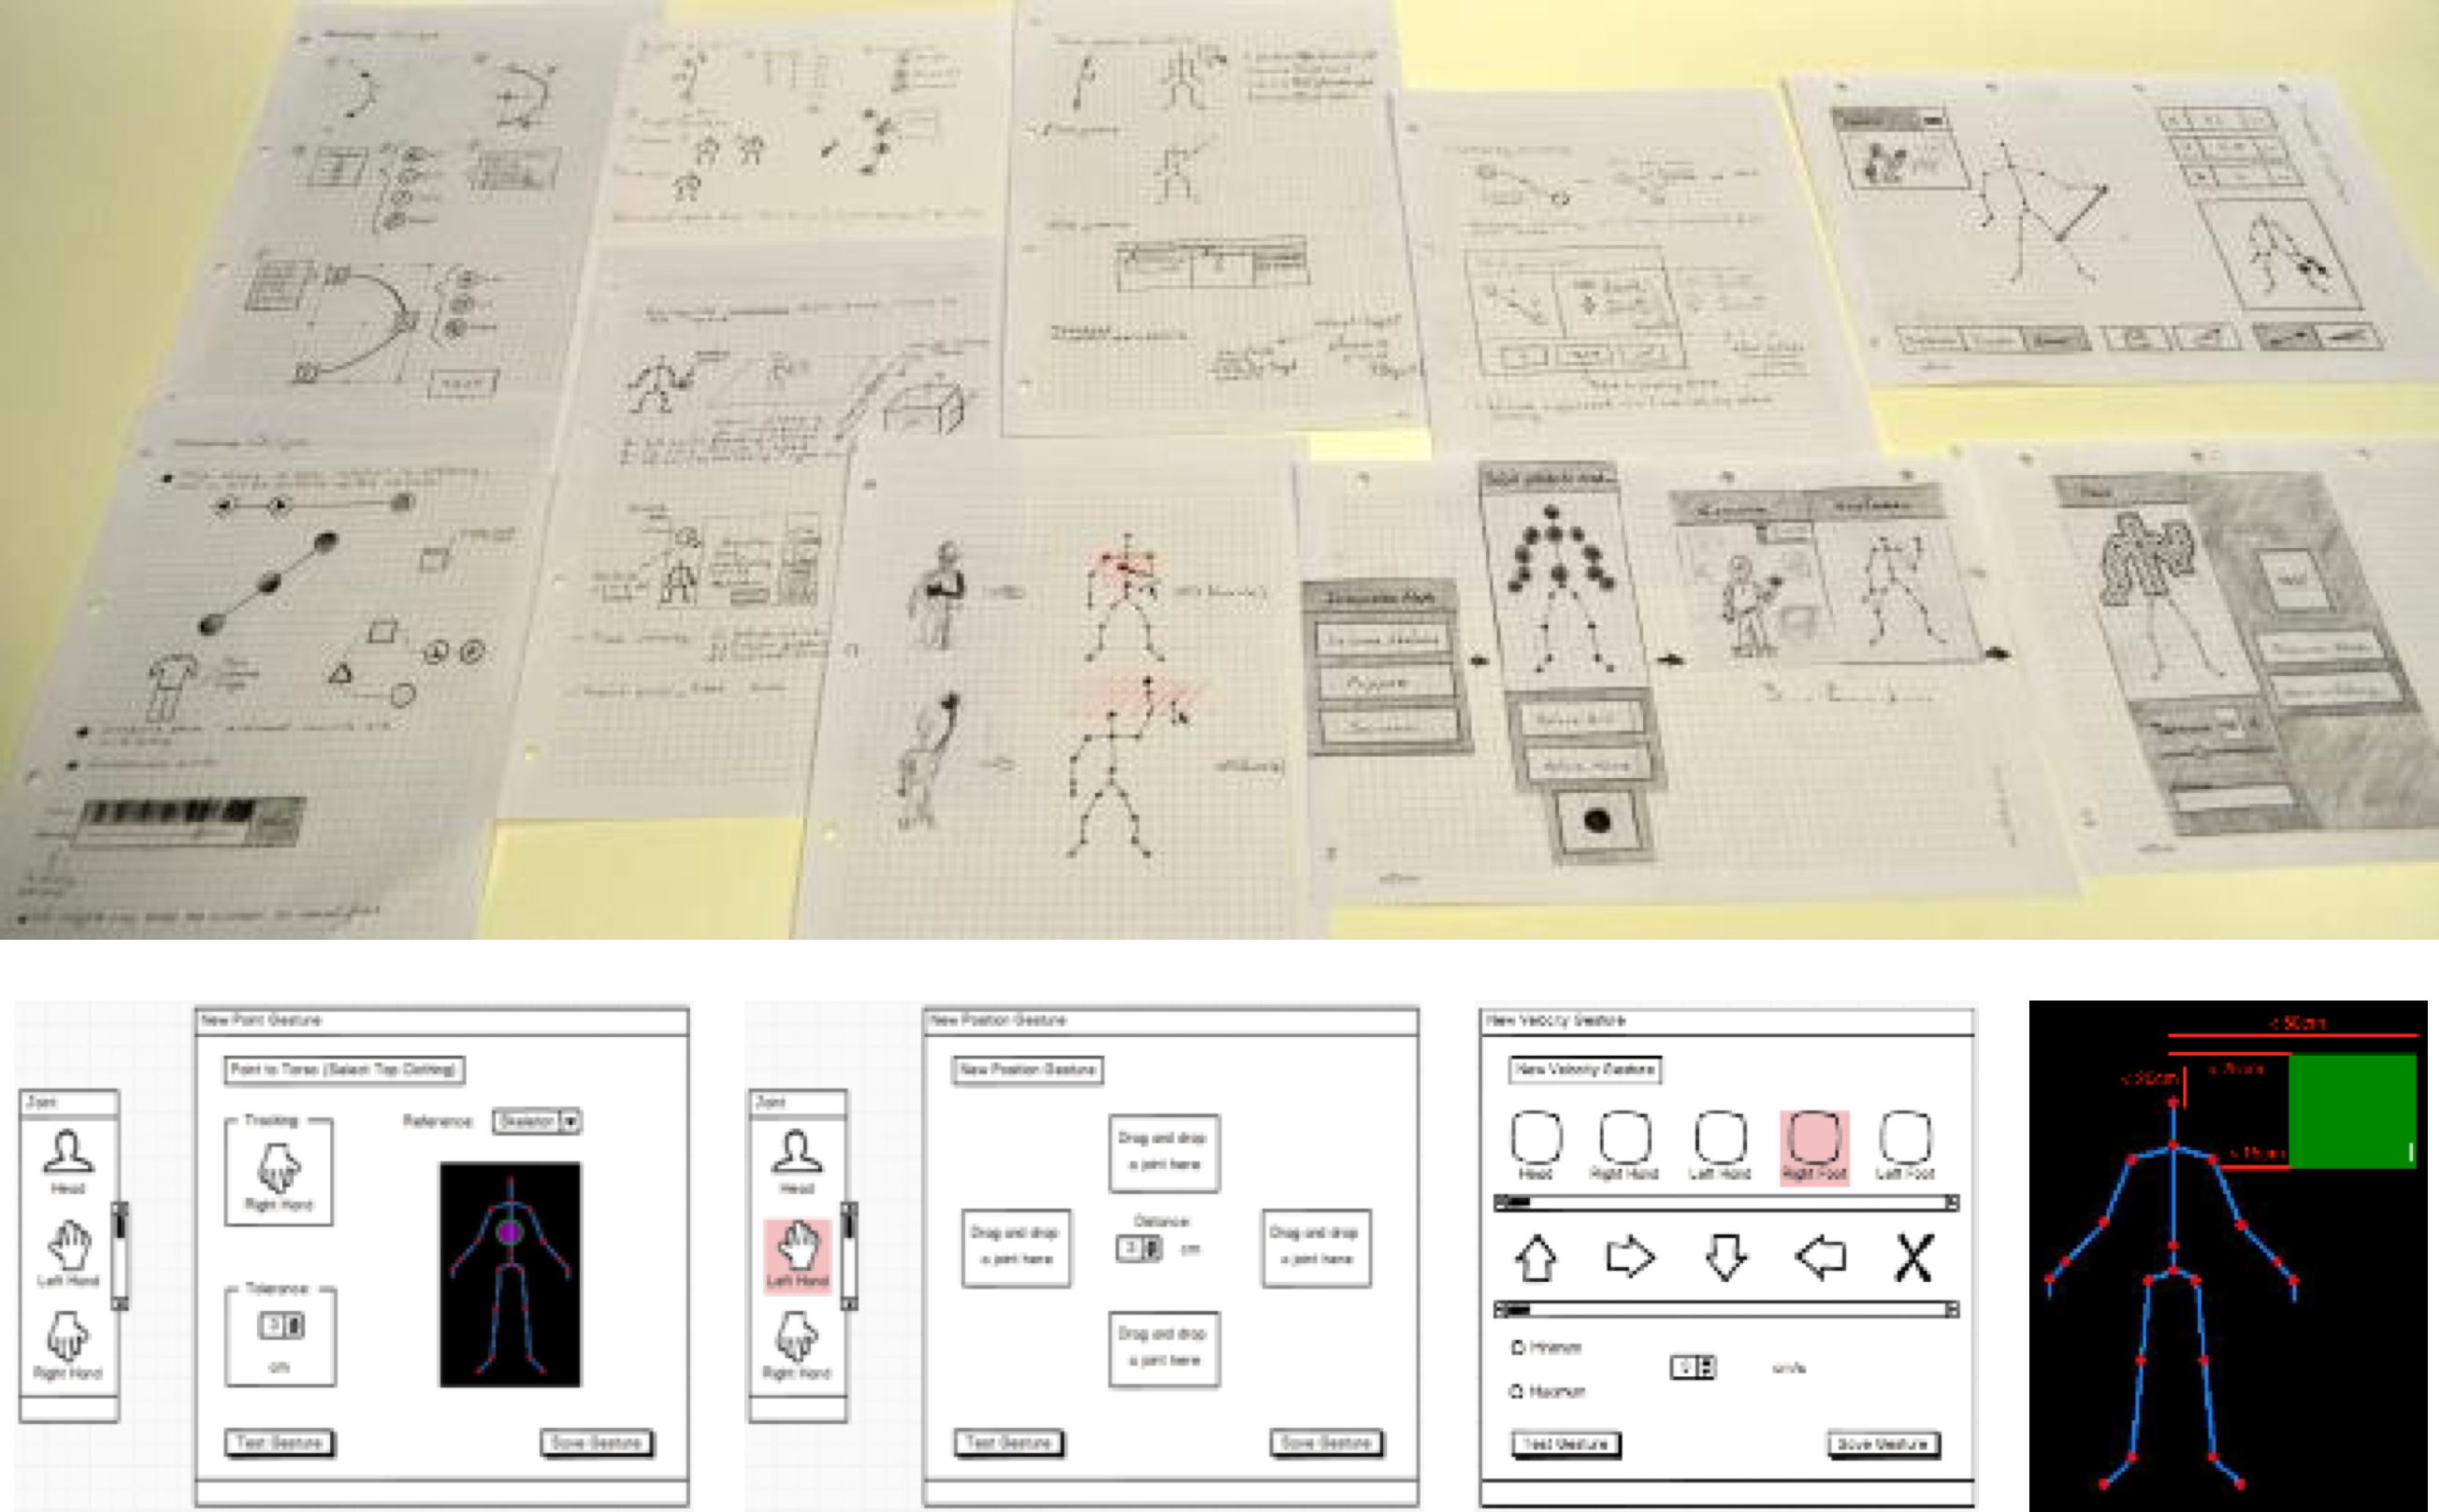
\includegraphics[width=\textwidth]{sketches-prototypes}
\caption{Rough sketches, paper prototypes, digital wireframes and interactive prototypes were used to gather feedback which directed design and development.}
\label{fig:sketches-prototypes}
\end{figure}

\subsubsection{Participants}

Participants consisted of a group of 10 potential users, aged 22-31 ($\mu$=26), from diverse backgrounds. While recruited from among students and staff of a single university and not representative of a wide demographic, they represented the target users of a gesture authoring tool well. Each had different skills and interests. Among them was an industrial designer, a semi-professional musician, an electronics engineer, a computer scientist, a museum studies student, an interaction designer, a psychologists and a legal consultant. All participants were regular users of desktop computing applications. They were all were self-reportedly familiar with mid-air gestural interaction in the context of gaming; though none had any familiarity with existing tools for authoring custom interfaces. Participants' profiles was appropriate for the aim of the study: to elicit desiderata for a tool that would enable "nonconsumers" \parencite{Christensen:2003, Fried:2008} by lowering the threshold for building custom gesture interfaces.

\subsubsection{Procedure}

Two meetings were conducted with the participants. Qualitative and semi-structured feedback formed the basis for the results obtained during these meetings.

\begin{figure}[t]
\centering
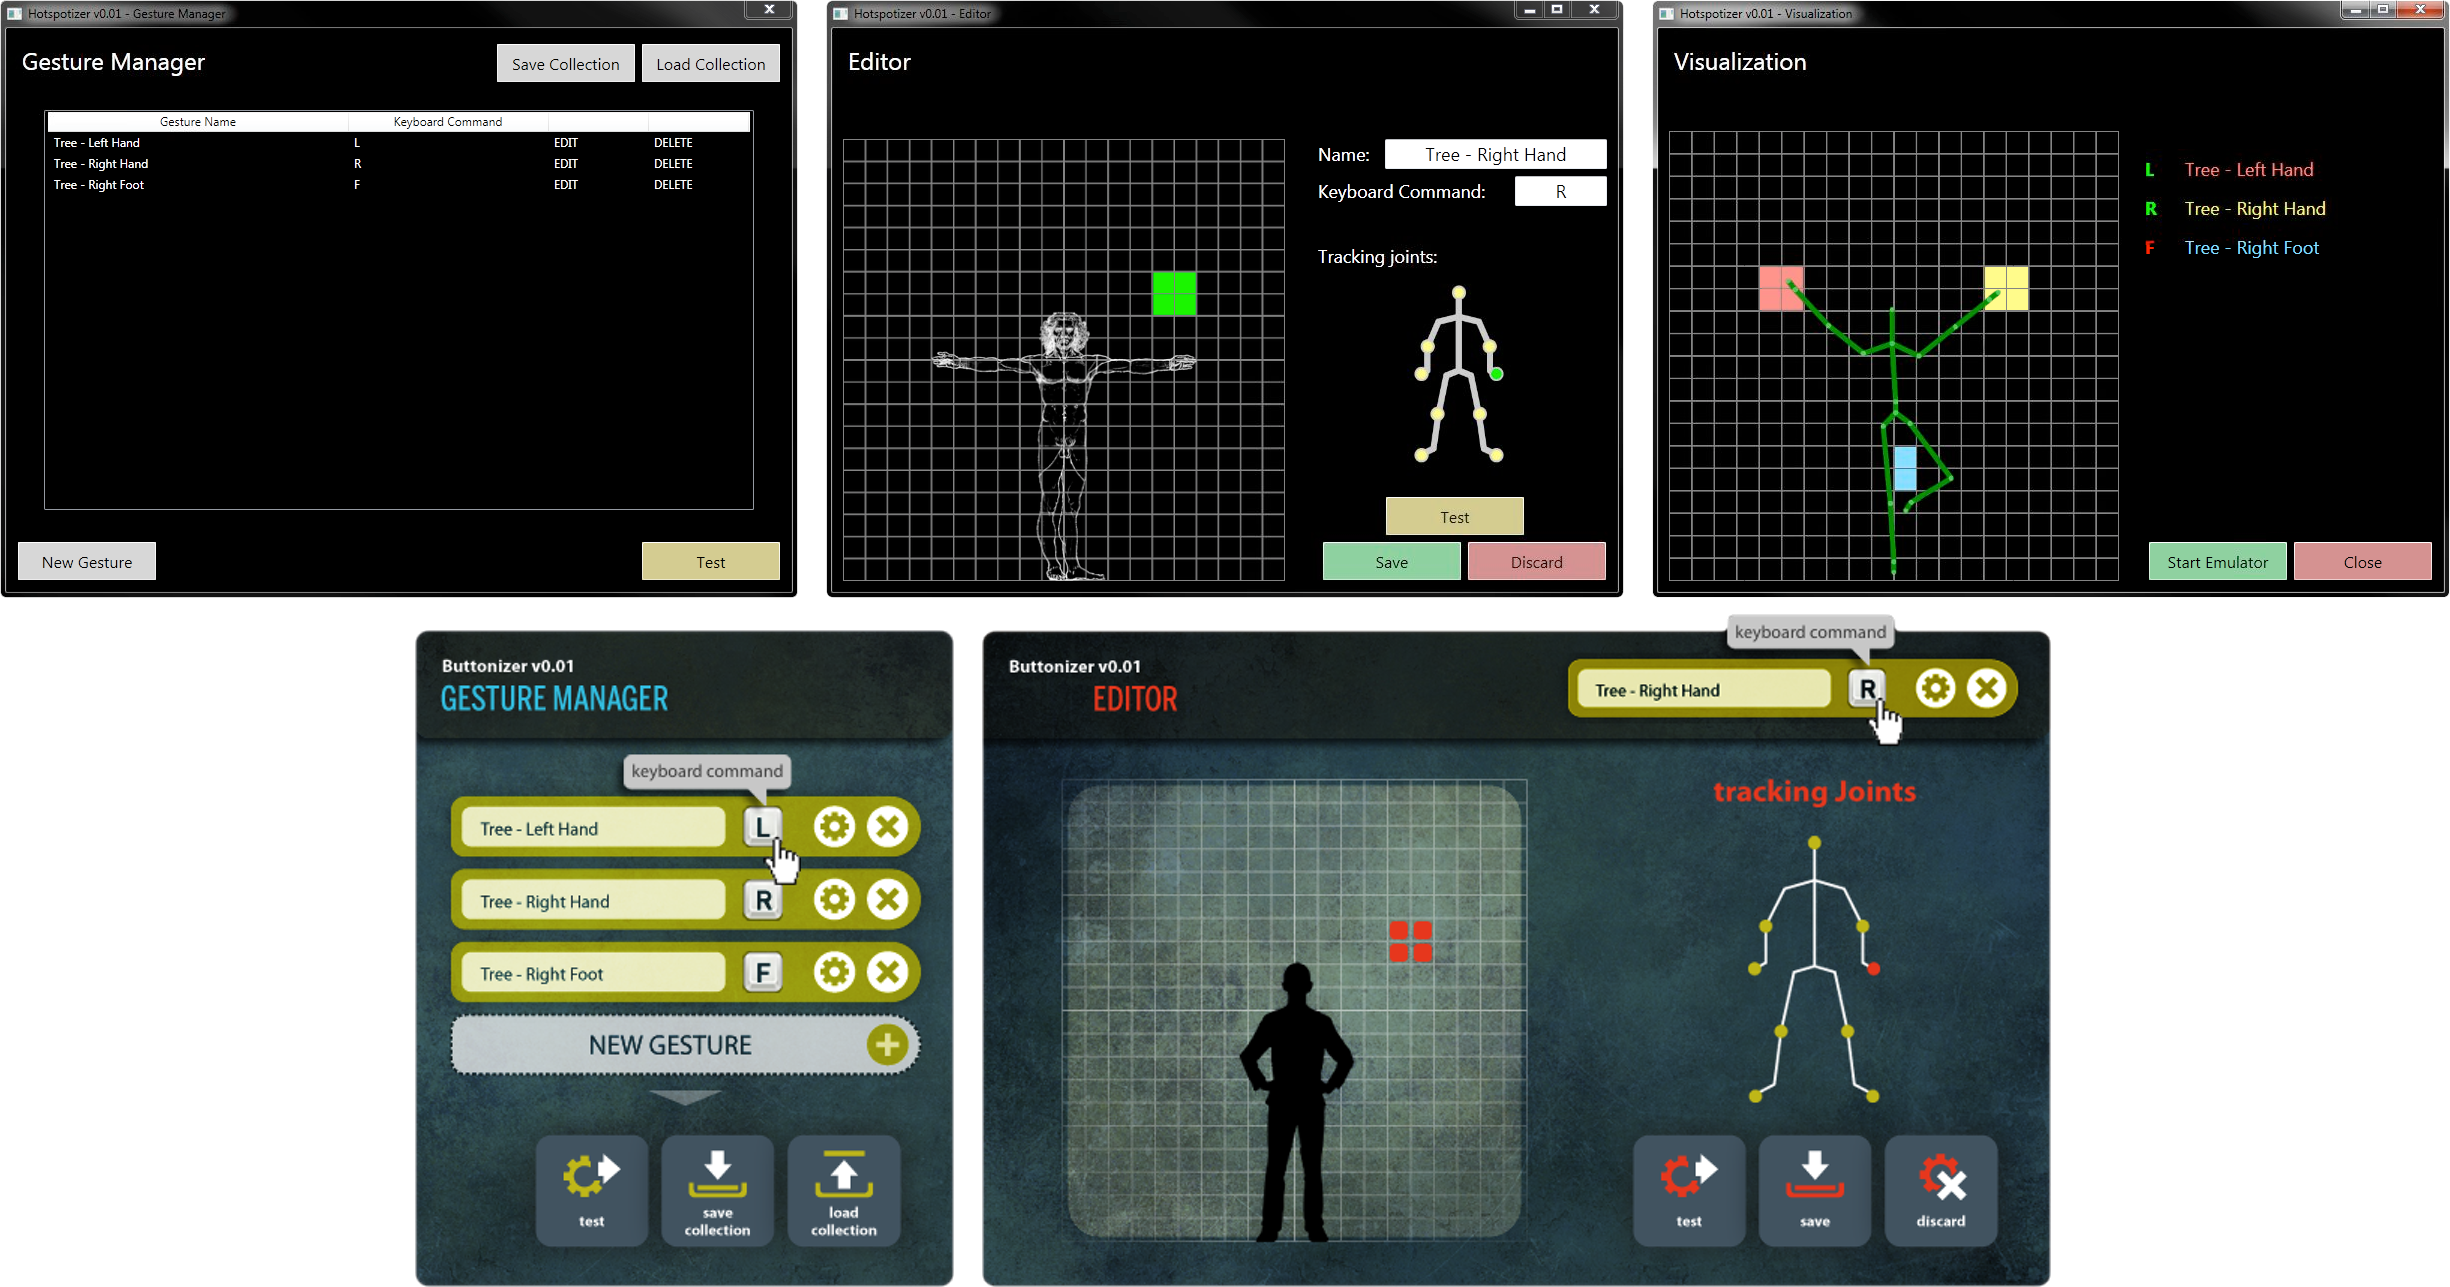
\includegraphics[width=\textwidth]{old-hotspotizer}
\caption{Early designs implemented rudimentary functionality and visually differed from the current user interface. Screenshots on the top row depict a very early prototype. The bottom row depicts a version with custom graphic design elements, later abandoned in favor of components native to the operating system.}
\label{fig:old-hotspotizer}
\end{figure}

During the first meeting, participants were given an introductory presentation on gestural interfaces, enabling technologies, and applications. Including this presentation, the meeting time slightly exceeded one hour. After the presentation, we discussed possible applications of gesture interfaces in participants' own domains of interest, with a focus on the use of mid-air gestures. Initial ideas for the design of a gesture authoring tool, in the form of rough sketches and paper prototypes, were presented to the participants. These initial prototypes were inspired by design considerations derived from the literature (see Section~\ref{sec:design-and-evaluation-of-tools}) and previous works on tools for authoring mid-air gestures (see Section~\ref{sec:authoring-mid-air-gestures}). Feedback collected from participants regarding the initial prototypes formed the basis for a second round of concepts.

Another round of sketches and prototypes was prepared, some of them higher fidelity; e.g. as a mock screencast showing the use of various modules in a gesture authoring suite, video sketches depicting a gesture authoring process based on programming by demonstration (see Section~~\ref{sec:authoring-mid-air-gestures}), and interactive user interface prototypes realized with \emph{Processing}. Knowledge derived from the comments and reactions of the participants to these concepts culminated in the construction of a prototype application with rudimentary features. This application implemented a simple version of the space discretization paradigm for authoring mid-air gestures, which was identified during the course of the second meeting.

\subsubsection{Results}

Early concepts that were presented to focus group participants included an end-to-end environment for creating gesture-controlled interactive movies that fused gesture authoring and content creation in one application; ready-made widgets that pre-implemented gesture control and plugged into existing development and design environments; and tools to overlay information (such as the distance between two specific joints) onto a visualization of a skeletal model, to complement textual programming. Discussions on possible applications for custom gesture control revealed that a modular approach that can interface with a diverse variety of applications is preferable to a full-blown content creation suite. Moreover, even among users engaged in design or programming activities, tools used for these purposes varied greatly. This illustrated the value of a standalone application rather than a tool that generates code in a specific programming language or plugs into a specific environment.

The idea of creating virtual buttons or hotspots in the space around the user and using them to define gestures was depicted in the sketches that were shown in the second meeting, as well as an interactive mockup developed in \emph{Processing} (see Figure~\ref{fig:sketches-prototypes}). Other ideas included an application that recognized static poses and a graphical language consisting of atomic primitives for composing gestures. Here, the concept of space discretization was proposed by a participant, an interaction designer. Upon interacting with the mockup of an interface where free-form areas in space can be made into gesture-tracking hotspots, she commented that she often makes use of squared paper when sketching. Instead of defining free-form regions in space, why not divide space into squares and constrain hotspots to these squares? Further discussion with participants revealed that this paradigm is grasped more easily than composing with atomic actions or constraints, or even demonstration. Moreover, using a visualization of the skeletal model and the space around it allows direct manipulation \parencite{Hutchins:1985}; encapsulates the limitations and prospects of the design space; capitalizes on proprioception; and can mediate interaction through a tight feedback loop \parencite{Wilson:2012}.

Hotspotizer was developed as an implementation of this \emph{space discretization} paradigm yielded by these workshops. The design guidelines derived from \textcite{Olsen:2007} and \textcite{Shoemaker:2010} informed initial prototypes. They were also used as filters that transformed the findings from the formative studies into a concrete user interface design. The decision to map gestures to key press events from an emulated keyboard was grounded in \posscite{Olsen:2007} principle for building on an infrastructure that is common across users and situations. The use of the user's centroid --- rather than the Kinect sensor itself --- as the origin for the grid of hotspots functions as a binding between personal and extrapersonal space and leverages the user's sense of proprioception. Adherence to the remaining three design considerations guided the use of focus groups and user studies as design tools.

\begin{figure}[t]
\centering
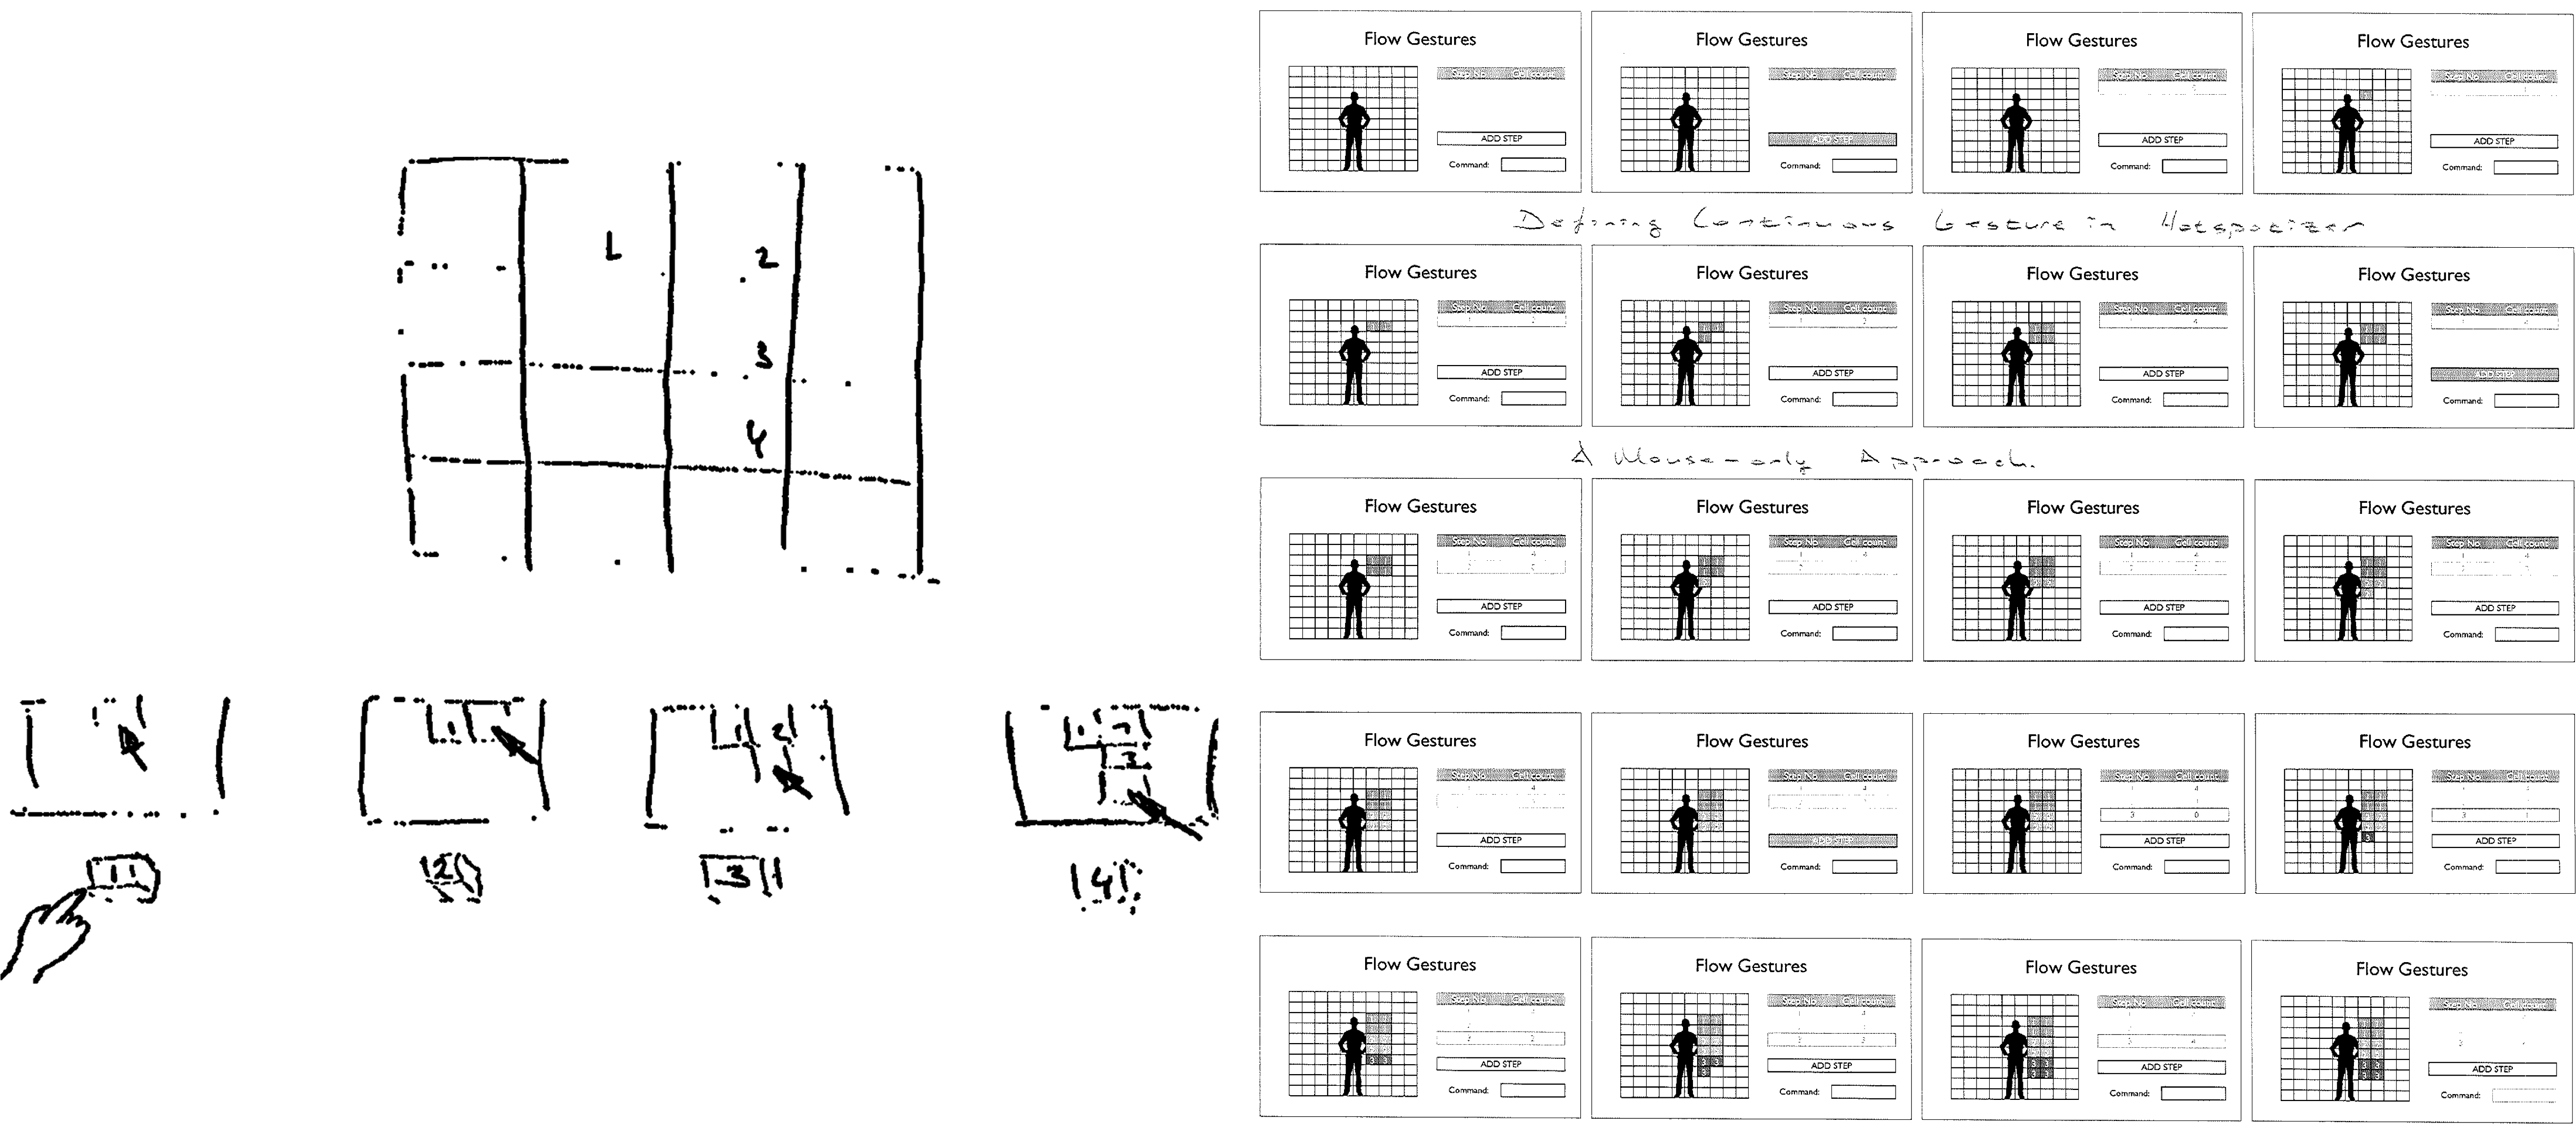
\includegraphics[width=\textwidth]{flow}
\caption{Rough early design sketches and higher fidelity wireframes were used to reflect on the workflow and user interface components for visualizing and authoring dynamic movements of human limbs.}
\label{fig:flow}
\end{figure}

\section{User Interface Design}
\label{sec:user-interface-design}

The knowledge on user needs, abilities, and preferences uncovered during the formative studies, along with insights derived from the analysis of gesture authoring software developed previously for both research and commercial purposes, has been utilized in the construction of the user interface for Hotspotizer. Design insights from previous works were collected from both previously published research findings, and from experience in using the artifacts. (Section~\ref{sec:authoring-mid-air-gestures} describes these efforts.)

The initial prototype featured only 2-dimensional gesture authoring capability, ignoring the depth component and tracking motion in the horizontal and vertical dimensions only. No key combinations were allowed, gestures could only be mapped to single key presses. There are also significant differences in the functionality and visual design of the user interface between this preliminary prototype and the final application. Two iterations on the interface design are shown in Figure~\ref{fig:old-hotspotizer}.

Following the initial stripped-down prototype, new features such as manipulating 3-dimensional spatial constraints and defining movement by using a timeline of keyframes (Figure~\ref{fig:flow}) were added to the application. Each feature underwent an iterative design and development process; beginning with rough sketches, evolving through prototypes of increasing fidelity, and finally culminating in the implementation (Figure~\ref{fig:prototypes}).

Beside tools for authoring gestural interactions (see Section~\ref{sec:authoring-mid-air-gestures}), a wide range of software and tangible design tools inspired the composition of the user interface. The interaction style for the main workspace for authoring 3-dimensional constraints using front- and side-views was inspired by 3D modeling software, along with architectural and engineering drawings (Figure~\ref{fig:architectural}).

The current version of the user interface is discussed in a detailed manner in Chapter~\ref{chp:hotspotizer}.

\section{Summative Studies}
\label{sec:summative-studies}

To evaluate Hotspotizer in use, two studies were conducted. The first was a study with 5 users to assess if Hotspotizer conforms to its design rationale. The second was a class workshop with 6 students working in pairs to build interactive prototypes of gestural interfaces. Qualitative results from these summative studies \hl{confirm that Hotspotizer conforms to its design rationale} Figure~\ref{fig:design-guidelines-satisfied} summarizes the observations that relate to the design guidelines, and the pertinent details are discussed below.

\begin{figure}[t]
\centering
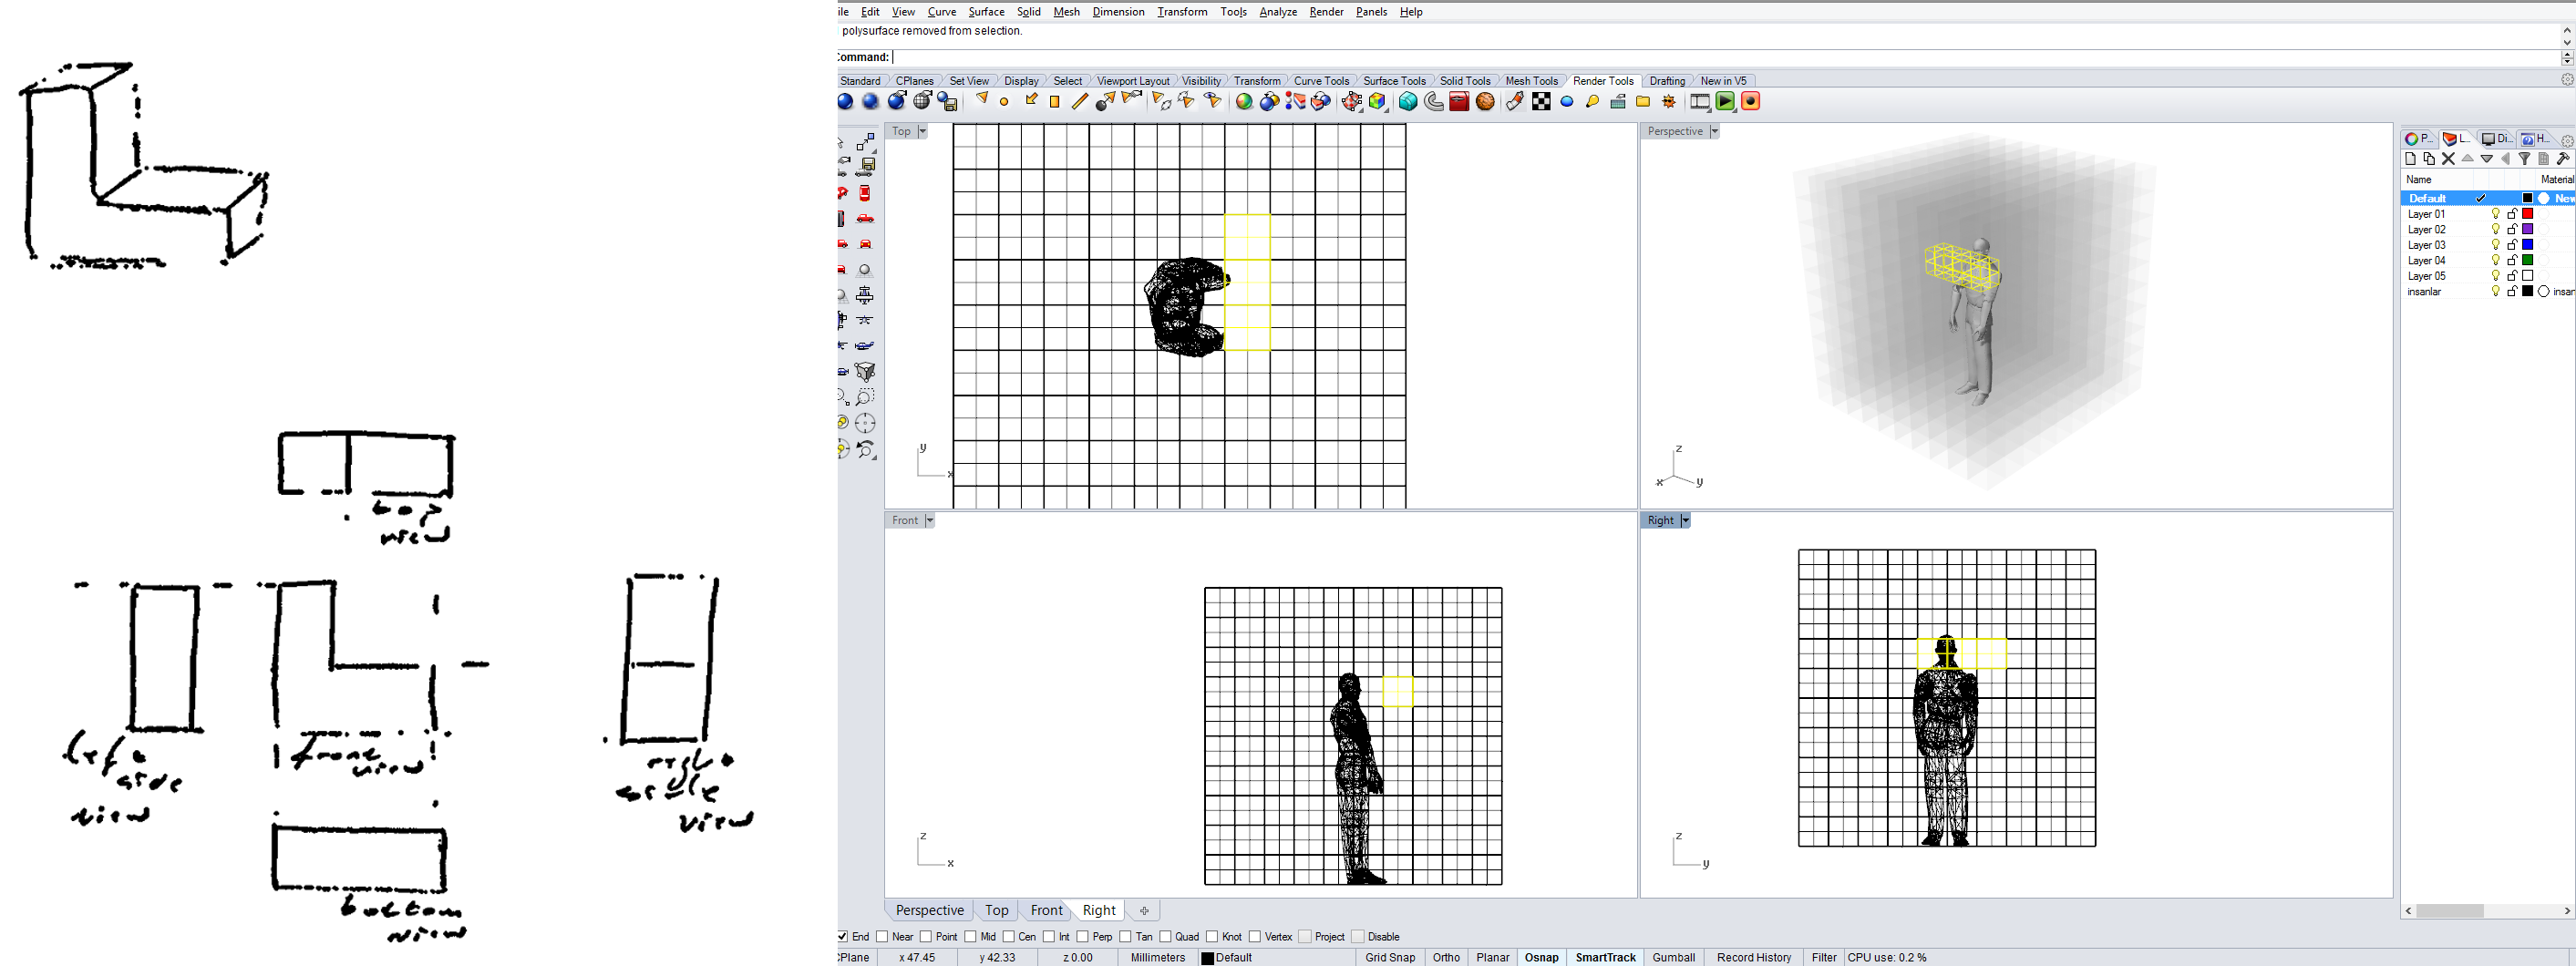
\includegraphics[width=\textwidth]{architectural}
\caption{User interface components for visualizing and manipulating 3-dimensional spatial constraints using front- and side-views was inspired 3D modeling software and technical drawings for expressing architectural and engineering designs.}
\label{fig:architectural}
\end{figure}

\subsection{User Study}

\subsubsection{Participants}

For the user study, five graduate students from a single university were recruited: an industrial designer, a museum studies student, a computer scientist, a psychologist and an interaction designer. These were not the same people who participated in the previous workshops. Participants were given a pre-study questionnaire where, on average, they self-reported a low level of experience with computer programming ($\mu$=2.1 on a 5-point Likert scale) and a low-medium level of experience with using mid-air gesture-based interfaces ($\mu$=2.4).

\begin{figure}[t]
\centering
\includegraphics[width=\textwidth]{prototypes}
\caption{Rough early design sketches and higher fidelity paper prototypes were used to reflect on the workflow and user interface components.}
\label{fig:prototypes}
\end{figure}

\subsubsection{Procedure}

Participants were given the task of adapting a non-gestural interface for a computer game to gesture control. They were provided a PC with a Kinect sensor. The game that was to be adapted for gesture control was a side-scrolling platformer --- this style of game was selected since users were expected to be fully familiar with the game mechanics and not be distracted from the process of gesture authoring. The participants were not given specific gestures to implement, but the game required three commands to operate: \emph{left} and \emph{right} for movement, and a \emph{jump} command. Participants were required to play through and complete the first level of the game using gestures at the end of the study. Participants first finished one level of the game using a keyboard; and they were gave a demonstration of Hotspotizer before they began authoring gestures to control the game. Participants were not explicitly instructed to think aloud \parencite{Nielsen:1993:engineering, Holzinger:2005, Boren:2000, Jaspers:2004}, but they nevertheless made comments during the task, which were recorded along with observations on behavior.

\subsubsection{Results}

All five participants were able to complete the assignment successfully, within 5-14 minutes ($\mu$=7.4min) after being given the demonstration and left alone with the interface. Participants commented that the interface was \emph{“easy to use”} and \emph{understandable}.

Participants iterated rapidly over gesture designs --- for each gesture, they went through 2-6 ($\mu$=3) cycles of hotspotizing cells on the Editor and moving into the sensor’s range to test designs in person. Static hand positions were preferred for the \emph{left} and \emph{right} commands, while the \emph{jump} command inspired diverse gestures including kicking and nodding. A common error across participants was that they marked areas outside the reach of the arms and the legs.

Semi-structured post-study interviews revealed that users had gained insights about the workings of skeletal tracking gestural interfaces. Support for full-body postures such as jumping, along with compositions that involve multiple limbs and grab detection were reported to be desirable as additional features. This is in line with my vision for future work (see Section~\ref{sec:future-work}).

\begin{SCfigure}[\sidecaptionrelwidth][t]
\centering
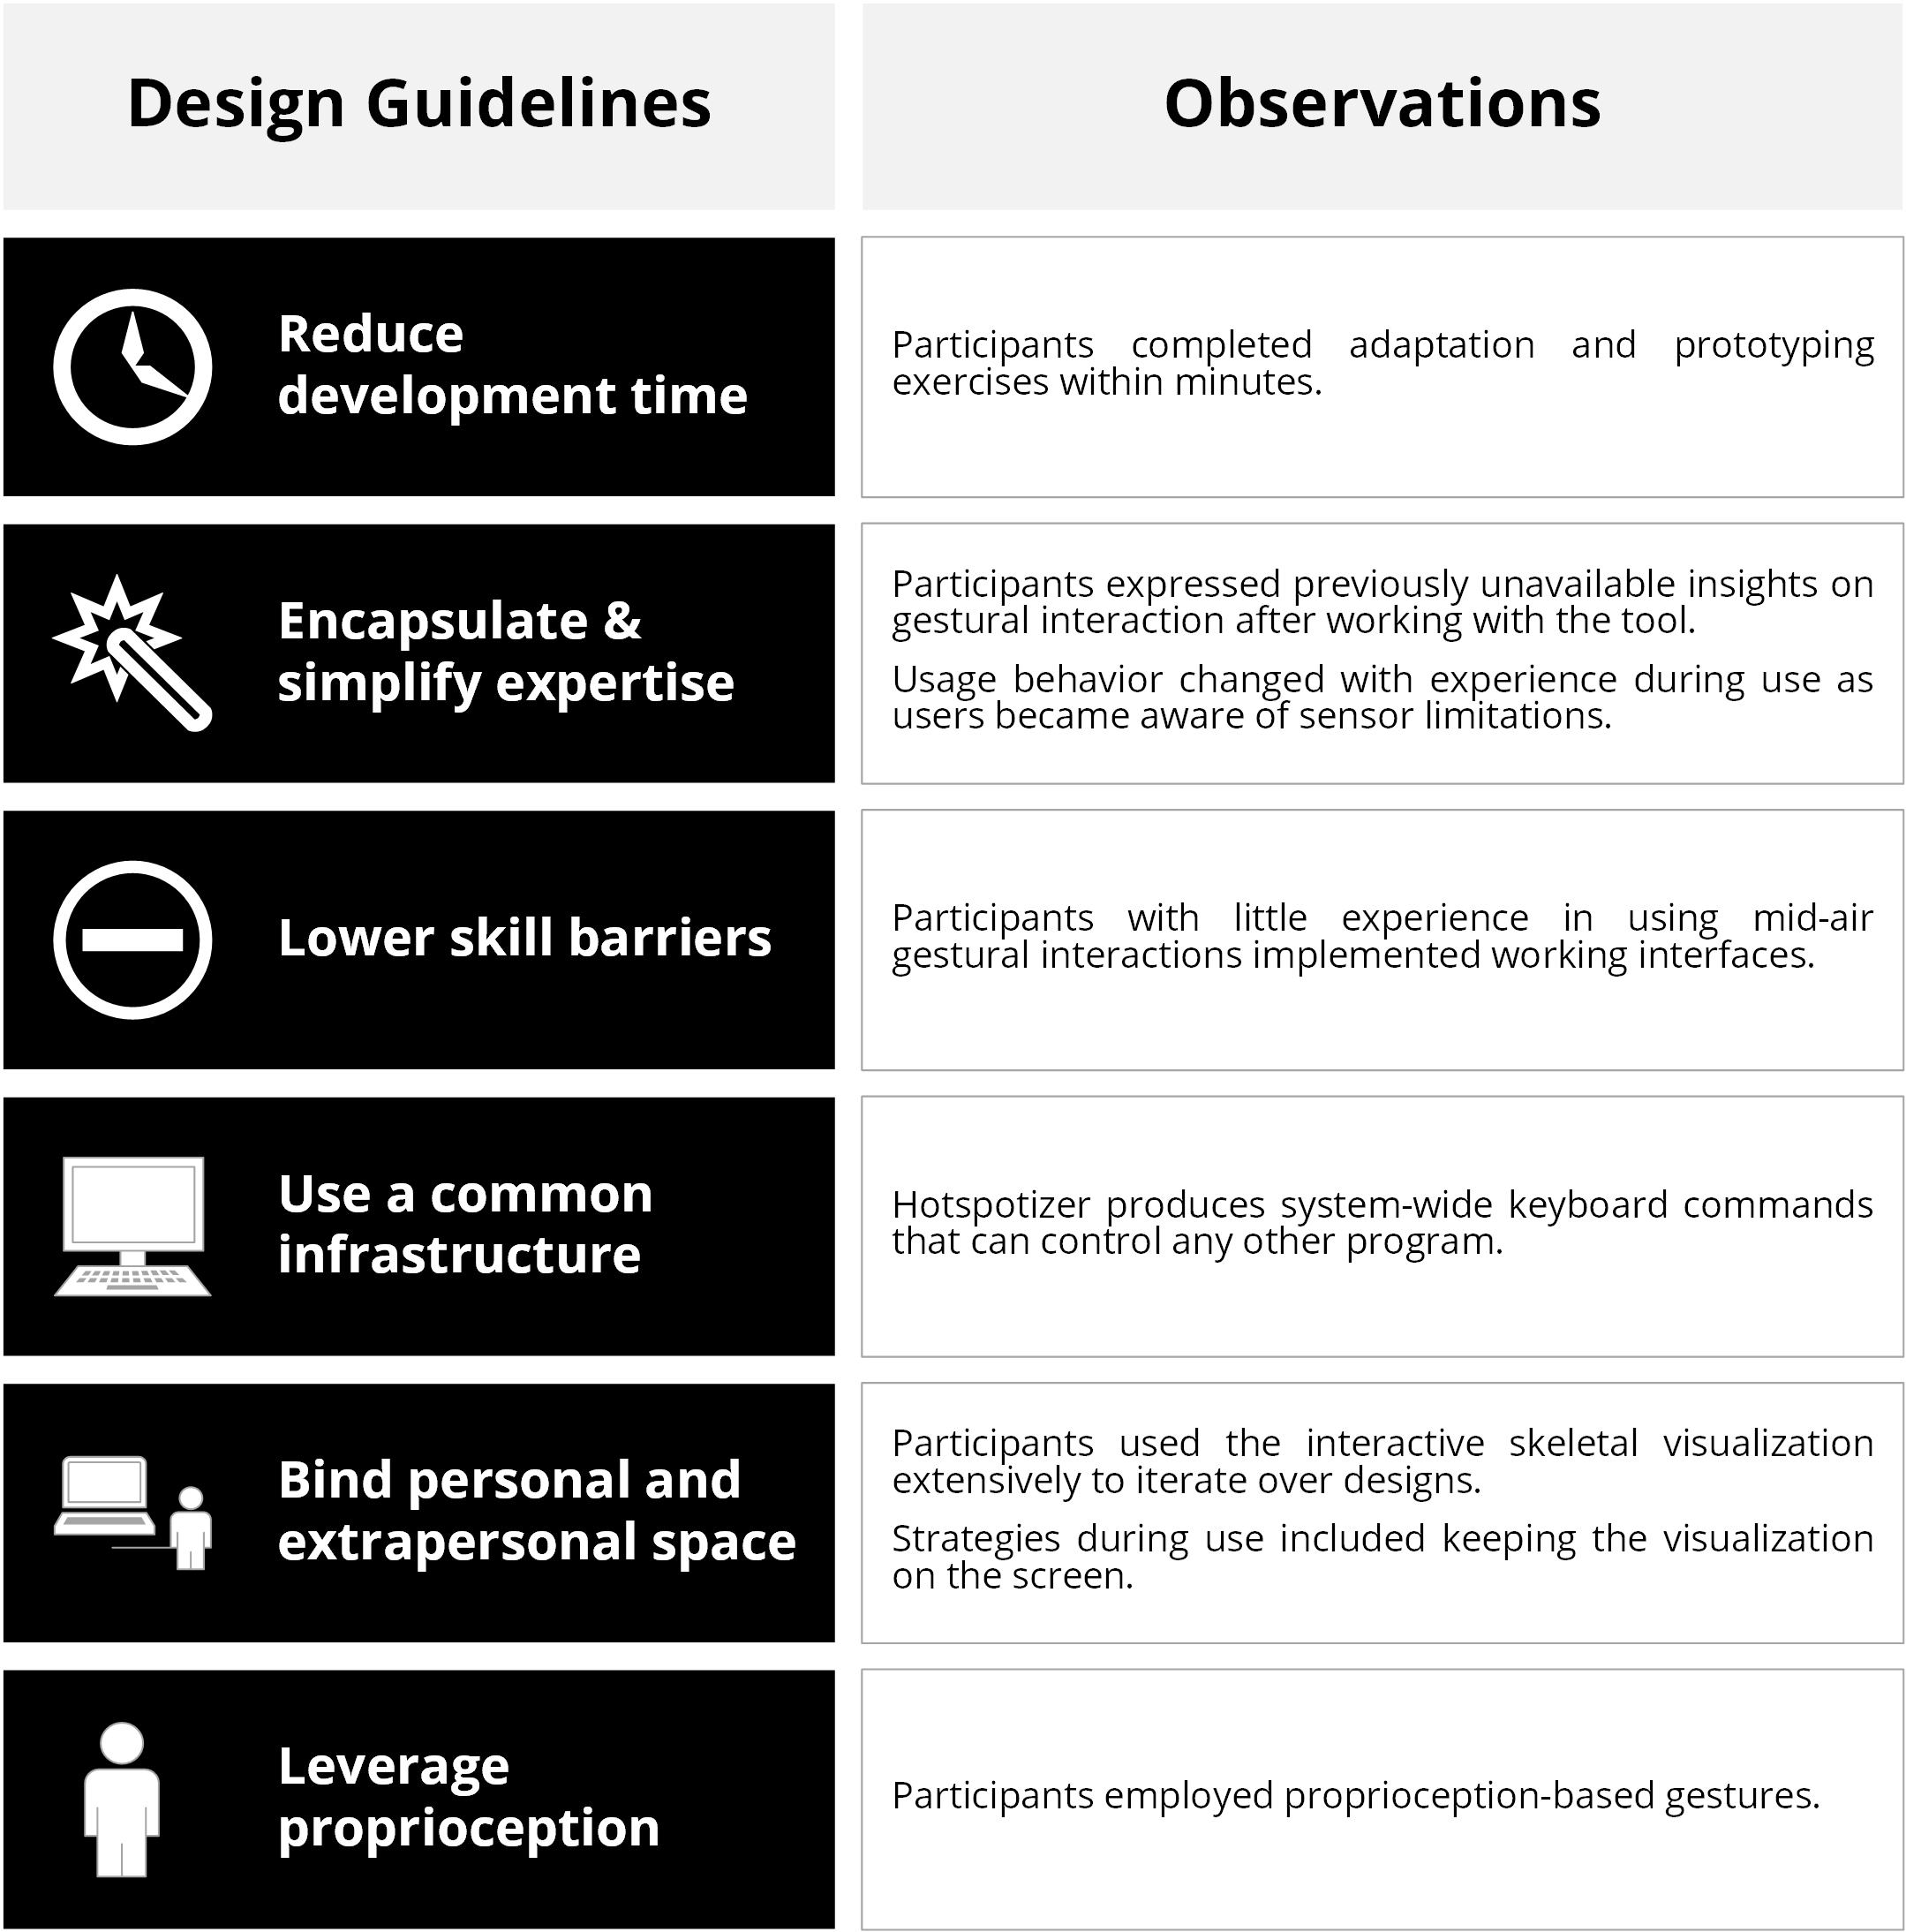
\includegraphics[width=.7\textwidth]{design-guidelines-satisfied}
\caption{Qualitative findings from two studies affirm that Hotspotizer is in keeping with our design rationale.}
\label{fig:design-guidelines-satisfied}
\end{SCfigure}

\subsection{Class Workshop}

\subsubsection{Participants}

The workshop was conducted with 6 graduate students who were taking a course titled “Design Thinking for Interactivity.” Participants worked in groups of two, with the three groups working the same time on different PCs.

All participants --- per course requirements --- were familiar with interaction design concepts and user interface prototyping processes. They self-reported low levels of experience with textual computer programming and using mid-air gestures to interact with computing applications outside of gaming ($\mu$=1.8 and $\mu$=2 on a 5-point Likert scale, respectively). One exception was a participant who claimed some understanding of software development concepts due to his experience as a graphic designer working on computer games, but even he did not have any programming experience. Again, per course requirements and the curriculum, participants were familiar with all of the software used during the study, except for Hotspotizer.

\begin{SCfigure}[\sidecaptionrelwidth][t]
\centering
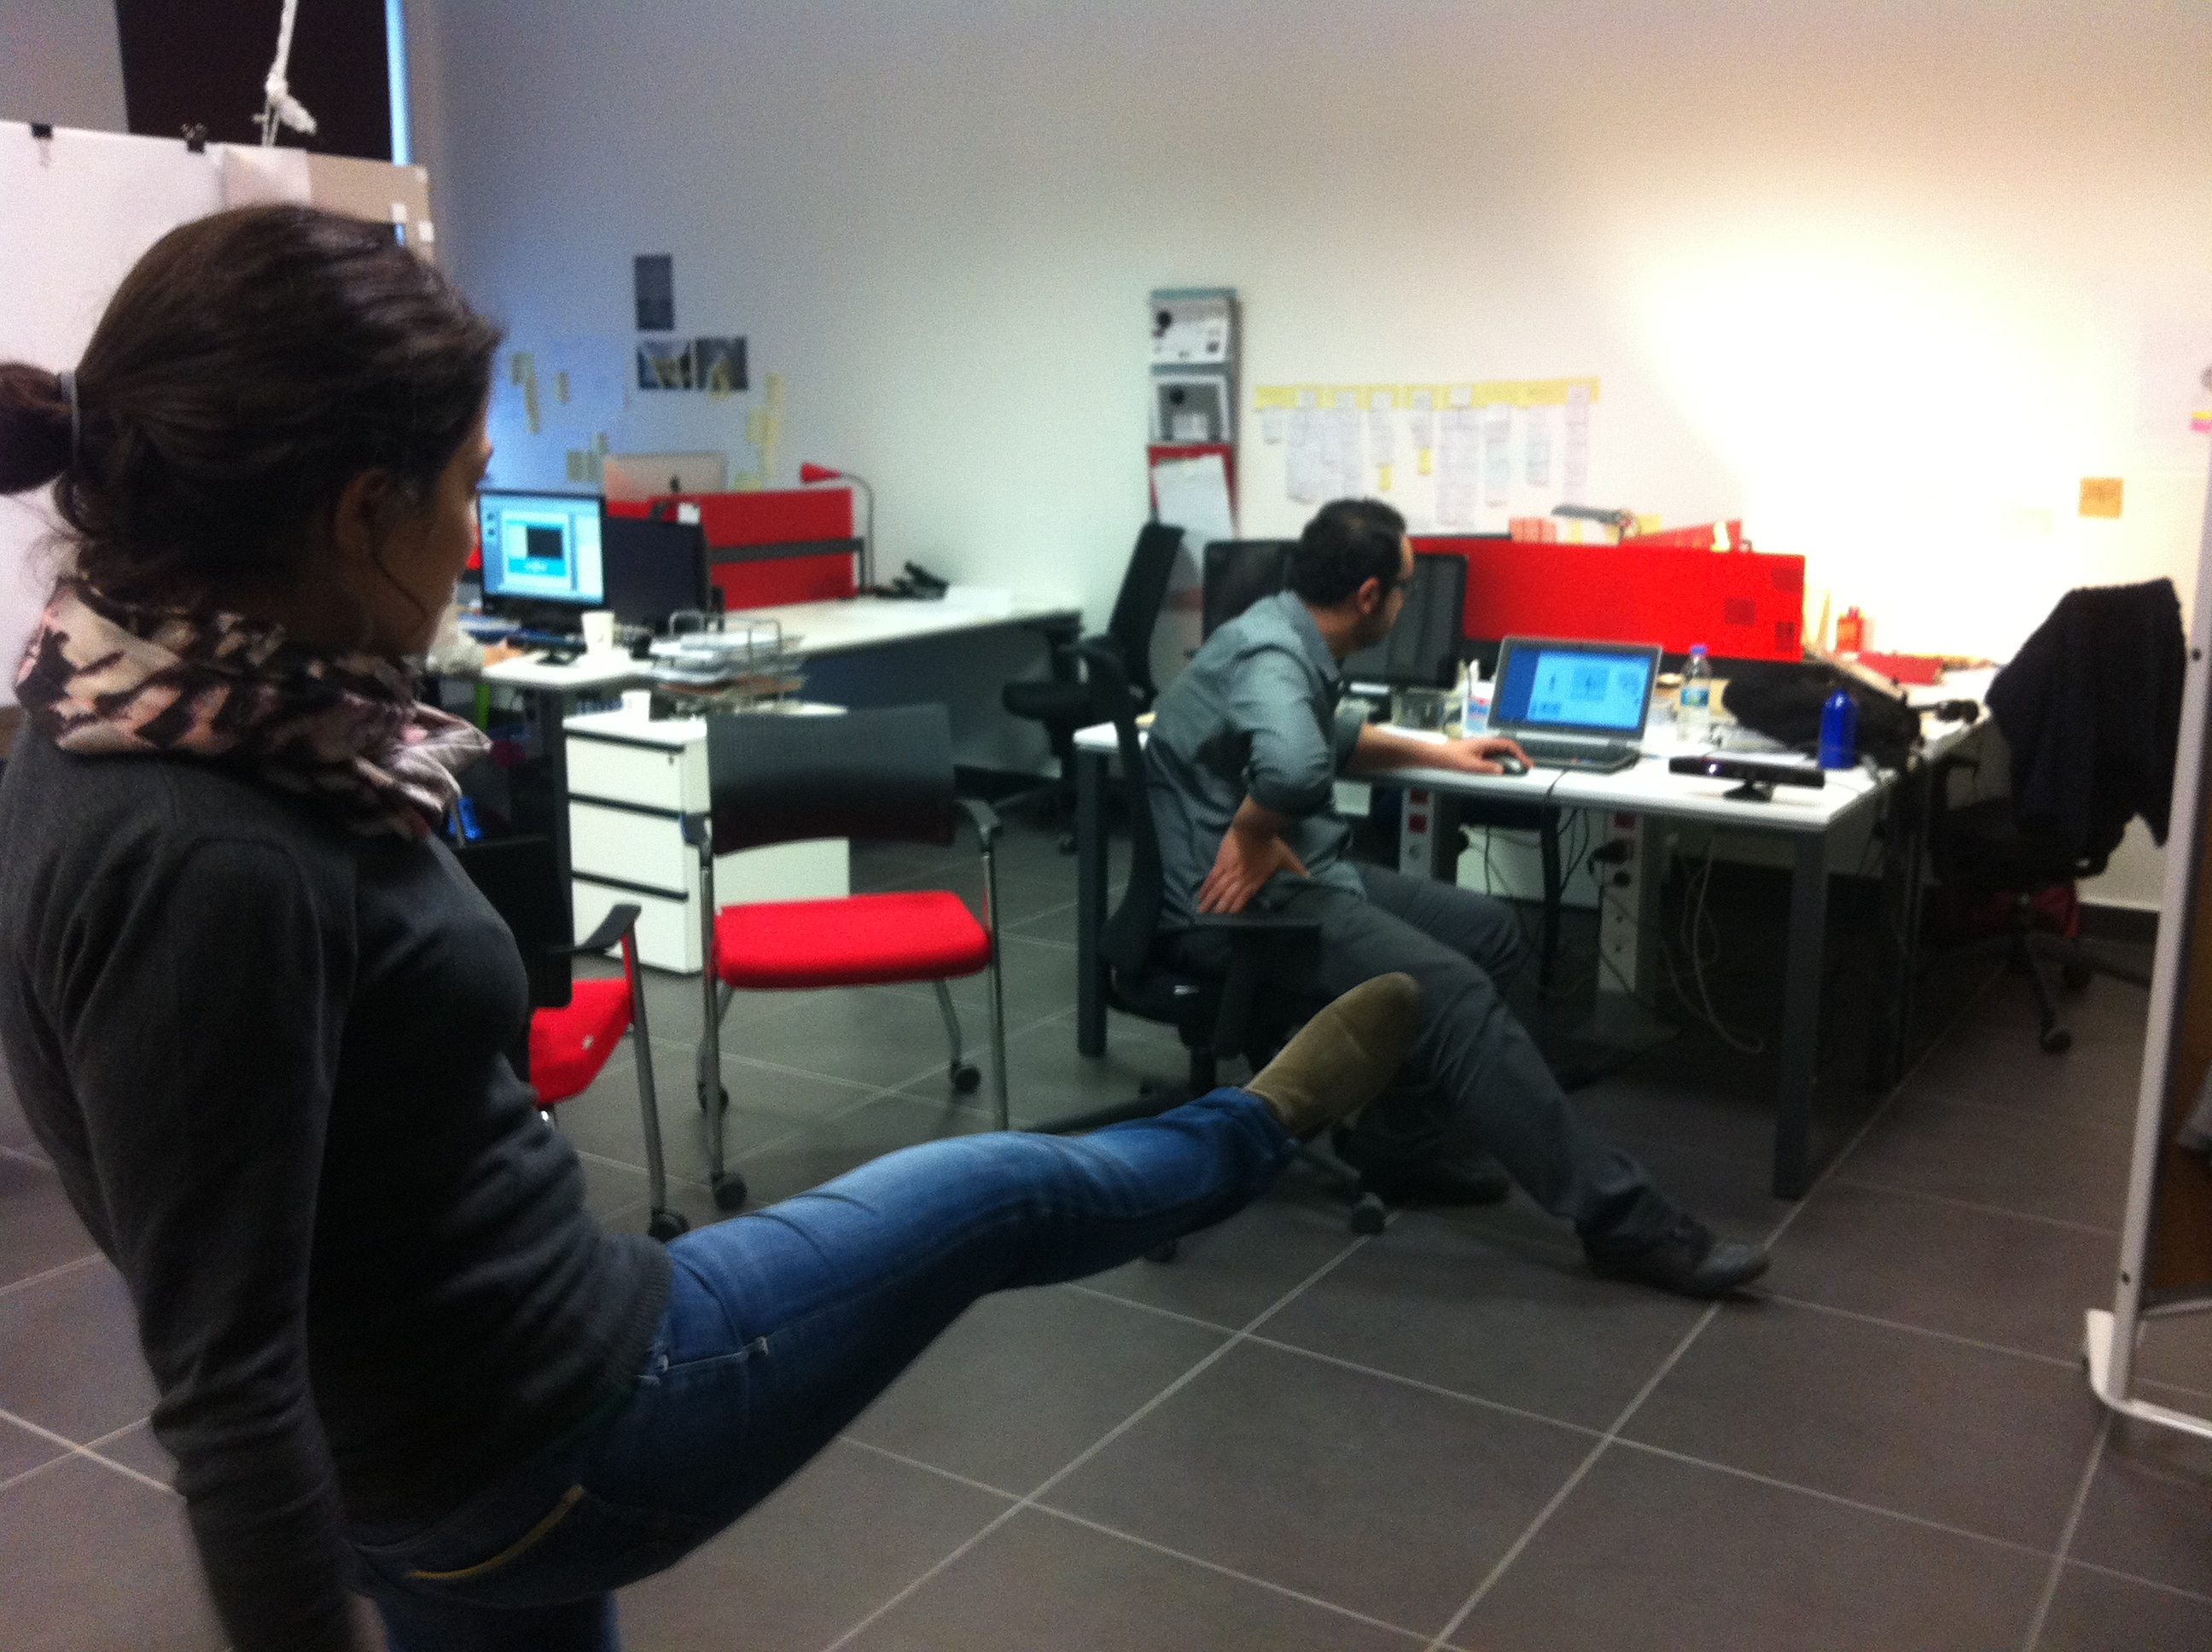
\includegraphics[width=.5\textwidth]{football}
\caption{User strategies included working in pairs. One user performs gestures in front of the sensor while the other marks hotspots that correspond to limb positions.}
\label{fig:football}
\end{SCfigure}

\subsubsection{Procedure}

The study began with a 20-minute presentation on how the Hotspotizer interface works. Participants were then tasked with creating interactive prototypes for three different systems (one per group) by following a single given use case for each system. The three systems comprised interactive digital signage for a movie theater, a penalty kick game and a video jukebox for public use. Participants were to create the visual design for the system’s screens in Microsoft PowerPoint\footnote{\href{http://office.microsoft.com/en-us/powerpoint/}{office.microsoft.com/en-us/powerpoint}}, and assign gestures to shortcut keys in PowerPoint to add interactivity. Each group was provided a Kinect sensor, a PC with Hotspotizer and PowerPoint installed, and a cheat sheet that exposed keyboard commands available in PowerPoint. A diverse set of interactions is possible in this manner, including moving between screens, starting and stopping video, adjusting the volume of the system, displaying versatile animations and automatically triggering timed behavior.

\subsubsection{Results}

All of the three groups were able to complete their implementations of an interactive prototype, from scratch, within the 60 minutes allocated for the activity. On average, about one third of this time was spent ideating and sketching designs, one third on composing visuals in PowerPoint and one third on authoring gestures with Hotspotizer.

The digital signage prototype was controlled by six hand gestures that involved pointing, swiping, pushing and pulling. The penalty kick game employed four gestures: kicking a ball towards the left, the right and the center; and making a large circle with the hand to restart. The video jukebox prototype was controlled by five gestures that comprised swipes and touching various parts of the head and the torso.

Participants expressed enjoyment from the process of creating interactivity and working with new interface technology. \emph{“A few days ago I did not even know that [mid-air gesture control] was possible. Now I just made my own working design,”} commented one participant.

Initially, users did struggle to understand the workings of the skeletal tracking. Two groups attempted to use gestures with minute differences that the Kinect sensor may not distinguish from each other, such as touching the eye with one finger versus touching the nose. Through trial and error, participants revised their gesture designs to match the capabilities of the sensor.

A limitation to the space discretization paradigm was expected to surface: Hotspots configured for one user could be inappropriate for another user due to differences in body size. After the three groups completed their projects, they tried out each other’s implementations to see if this was the case. The only time when gestures from a new user were not recognized was in the case of the football game, where large leg movements were involved. Differences in the length of the legs hindered gesture recognition across users. Tuning the gesture design to involve larger hotspot areas alleviated the problem. When using hand gestures, no issues were apparent.

When working in pairs rather than alone, users adopted a different strategy when editing gestures: A single user would mark hotspots using the static on-screen silhouette of a human body as a reference and then test using the interactive representation. Working in pairs, one of the users preferred to stand in front of the sensor and perform gestures, while the other watched the moving representation on the screen and used it as a reference when marking hotspots (Figure~\ref{fig:football}). To allow a single user to enjoy the advantages of using the interactive skeletal model for authoring, future work can implement the ability to infer hotspots from demonstration, along with voice control to interact with the program from a distance (see Section~\ref{sec:future-work}).

Participants were interviewed after the study, where they suggested that while editing, being able to see where hotspots belonging to previously authored gestures reside could be beneficial. This visualization was later added into the Editor module in a later version of Hotspotizer.

\begin{SCfigure}[\sidecaptionrelwidth][t]
\centering
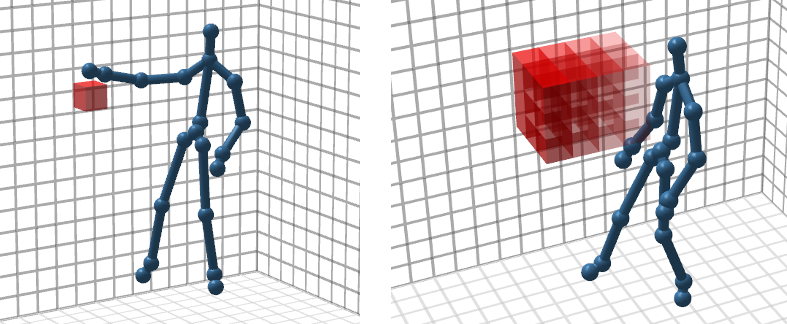
\includegraphics[width=.5\columnwidth]{constraints}
\caption{Initially, users preferred gesture designs that involved small hotspots and unspecified motion. Frames were added to constrain motion, and hotspots were enlarge to allow for variations during gesturing. Here, both panes depict hotspot configurations that may be used for a "punch" gesture. The configuration on the right is more conducive to robust recognition because of its sequentially constrained and spatially relaxed nature, compared to the rather extremely simplistic design on the left.}
\label{fig:constraints}
\end{SCfigure}

\subsection{Generalizable Observations}

During the summative studies, observations that are relevant for the design of mid-air gestural interfaces in general were encountered.

Users who self-reported little experience with mid-air gestural interfaces (a vast majority among participants) tended to be unaware of the limitations regarding the sensor’s field of view. This manifested as an initial tendency to stand too close to the sensor and perform gestures in areas outside the sensor’s field of view. Within minutes, users adjusted to become aware of the boundaries of the interaction area. To promote users' awareness of the depth sensor's field of view, the depth map provided by the sensor could be displayed on screen, as opposed to displaying the user's skeleton alone.

As they tested and used their own gesture-controlled designs, users tended to keep the Hotspotizer interface open and utilize the on-screen representation of the human skeleton. This confirms that the requirements for including a tight feedback loop and a representation for reporting the user’s actions within space are justified. Based on this observation, I can recommend that interfaces based on mid-air gestures include a representation of the tracked skeleton(s).

In general, when designing gestures, users preferred to start with static poses or specify only the end point of a gesture trajectory, utilizing only one frame to implement their designs. In simple cases, such as in controlling the side-scrolling platformer, these designs did suffice. However, as the quantity and complexity of gestures in the interface increases, this approach results in a high number \emph{false positives} in gesture recognition due to intermediate movements intersecting hotspots. Users, due to inexperience, did not anticipate this. Through trial and error, gesture designs were revised and conflicts were resolved, by adding frames and authoring \emph{movement} further constrain designs. Often, gesture designs resulted in \emph{false negatives} due to spatially overconstrained designs that involved small volumes, requiring precise and accurate performance of gestures. Participants, through trial and error, revised their designs by enlarging hotspotized \emph{volumes} to allow for some degree of ambiguity when performing gestures. The general tendency among users was to initially design gestures that were temporally or \emph{sequentially underconstrained} and \emph{spatially overconstrained}. Designs that minimize conflicts by \emph{introducing sequential constraints} (i.e. more frames) while allowing for some flexibility by \emph{relaxing spatial constraints} (i.e. more hotspots) were observed to be more conducive to robust recognition (see Figure~\ref{fig:constraints}).

\subsection{Discussion}

\textcite{Olsen:2007} reasons that conventional structured usability evaluation methods are not appropriate for novel user interfaces and design tools in particular; since they violate three important assumptions of usability testing:

\begin{itemize}
\item \emph{"Walk up and use."} The first assumption is that the system being evaluated must be operable with minimal training. This holds for tools intended for a very wide non-expert user base --- e.g. home appliances --- and for tools that target a population with "shared expertise" --- e.g. doctors or teachers. User interface design, Olsen argues, requires "specialized expertise" which will vary highly among participants recruited for a usability test, even among those belonging to the same profession.
\item \emph{The standardized task assumption}. "A task that is suitable for a usability experiment must have low inherent variability so that any variance can be assigned to the differing techniques being tested, not to variations in approach to the task or user expertise." \parencite{Olsen:2007} In other words, software built to support complex tasks involving a high number of steps and many solutions cannot be evaluated through conventional usability approaches. The design of gestural interactions is one such task.
\item \emph{Scale.} Due to economic and psychological issues --- e.g. participants' attention spans --- usability tests must be completed within 1-2 hours. The return on investment --- in terms of statistical significance --- for running lengthy and multiple sessions is low.
\end{itemize}

Olsen recommends design considerations and evaluation criteria for novel user interface tools, which were described in Section~\ref{sec:design-and-evaluation-of-tools} and used extensively to inform the design process for Hotspotizer. The user studies described in this chapter, while inspired by conventional usability tests in terms of the procedures followed, were conducted with a focus on obtaining qualitative results. Also in line with the approach recommended by \textcite{Nielsen:2000, Nielsen:2011}, and \textcite{Nielsen:1993}; I used usability-inspired procedures to uncover bugs and implementation errors in the system, elicit user strategies, inspire new features, evaluate the use and misuse of existing features, and determine if users can make sense of the user interface and the task in general. These efforts have proven valuable in informing design and development. In short, while I agree with Olsen that conventional usability testing with a quantitative focus is not a productive approach for the for novel interfaces; but usability methods could be adapted in these cases towards comparatively informal procedures that deliver qualitative feedback from real users. This feedback is highly valuable for user interface design.
